\chapter{Data Collection and Simulation} \label{chapter:data}

\section{Introduction}

    The amount of data output by the ATLAS detector is immense and overwhelming.
    Reading out every single bunch crossing would require phenomenal bandwidth and would take centuries to process.
    To counteract this overabundance of data, ATLAS relies on an on-site bunch crossing filtering system to drastically reduce its throughput.
    Known as the ATLAS trigger system, this critical piece of infrastructure constitutes the last step of data taking,
        and the first step of physics analysis.
        
    Having such a system in place is not by itself sufficient however,
        without guidance as to how it and its output should be utilized.
    Throwing out bunch crossings without reason will remove events of interest as often as irrelevant events.
    In order to make informed decisions as to how filtering should be done,
        data is not only collected from ATLAS, but is generated through Monte Carlo simulation processes.
    These simulated data samples provide insight into how different physics processes may present in ATLAS,
        allowing for greater efficiency in what data is kept, and what is removed.


\section{Trigger System}

    The trigger system is a series of hardware and software level algorithms designed to quickly identify bunch crossing ``events'' which may be of interest to physics analysis, while discarding the rest.
    Referred to as ``online'' analysis, these algorithms perform event selection live, in parallel to the ATLAS machine running and taking data.
    The trigger system processes all ATLAS events immediately after readout, ultimately reducing the 40 MHz bunch crossing rate to a data output rate of 1 kHz.
    The data which survives this rapid selection is read out to disk and distributed to individual research teams for more sophisticated ``offline'' analysis later.
    
    Triggering is achieved by running events through two sequential trigger systems.
    All events first go through the hardware-based Level 1 Trigger (L1) before being run through the more sophisticated (and slower) software-based High Level Trigger (HLT).
    Both of these triggers involve a plethora of different measurements on various aspects of the events, such as total transverse energy, transverse momentum, jet multiplicity, and opening angles between jets.
    All of these measurements are factored into whether or not an event passes the trigger selection.

    Each of the various kinematic properties checked by the triggers have multiple threshold values that can determine a ``pass.''
    For example, a jet $p_T$ trigger can have thresholds at 30, 45, or 55 GeV, among others.
    A ``trigger chain'' is a combination of several different such kinematic conditions, each with their own thresholds.
    A bunch crossing is ultimately accepted and read out to disk for further analysis offline if it is able to pass all the conditions of a trigger chain.
    There are hundreds of different trigger chains, each permitting different combinations of kinematics.
    An event is read out if it passes any one of these trigger chains, and is labeled in data with all the trigger chains it passes.
    The trigger chains used in ATLAS were decided upon before the beginning of the Run 2 data taking period, based on input from various analysis teams.
    This predefined list of trigger chains comprise what is known as the ``trigger menu'', and ultimately defines what kinds of physics processes ATLAS analyses have access to.
    The following sections describe broadly how the two levels of the trigger system work, and later chapters will focus on which trigger menu items are used in the di-Higgs analysis specifically .

    \begin{figure}[h]
        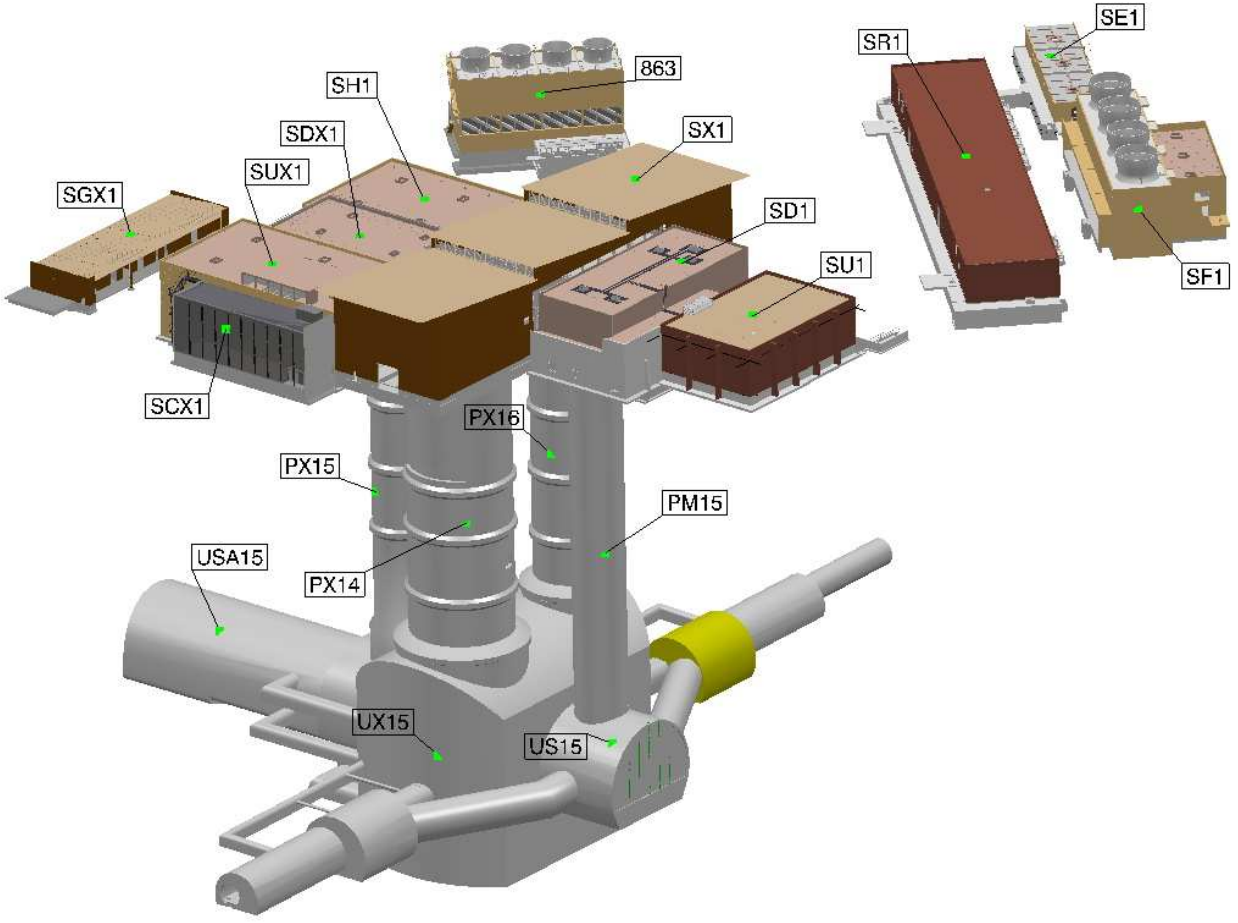
\includegraphics[width=\linewidth,height=\textheight,keepaspectratio]{trigger/facilities}
        \caption{General layout of buildings and facilities at LHC Point 1, site of ATLAS \cite{trigger_tdr}}
        \label{fig:facilities}
    \end{figure}


    \subsection{Level 1 Trigger}

        One bunch-crossing every 25 ns is a blistering pace to operate at.
        The first layer of the trigger system, L1, therefore must run entirely through hardware-level gate logic.
        The goal of this system is to reduce the event rate from the raw 40 MHz bunch-crossing rate, down to a more manageable rate of 100 kHz \cite{trigger_run2}.
        To reduce latency as much as possible, all the electronics comprising L1 are located as close as possible to ATLAS itself, specifically in the USA15 underground chamber \cite{trigger_tdr} (see figure \ref{fig:facilities}).
        As yet another consequence of the high frequency L1 must operate at, it exclusively uses information from the ATLAS calorimeters and Muon Trigger Chamber for its decisions.
        %(utilizes detector buffer memory to keep up).

        The Muon Trigger aspect of L1 is based entirely on the trigger-dedicated Muon Trigger Chamber, described in section \ref{sec:muon-trigger_chamber}.
        Its purpose is to make trigger decisions primarily based on muon $p_T$ and track multiplicity in the Trigger Chamber \cite{trigger_run1}.
        In the calorimeter-based trigger, the selection algorithm first requires a reduction in data resolution.
        The full granularity of the ATLAS calorimeters is too complex to analyze in the 25 ns L1 has to process each bunch-crossing.
        Instead, the various sensors of the calorimeters are clustered together into ``trigger towers'',
            each with a resolution of $0.1 \times 0.1$ in $\Delta \eta \times \Delta \phi$.
        The way towers are clustered and used varies between the different L1 calorimeter trigger modules: the CPM, JEM, and CMX.

        \begin{figure}[h]
            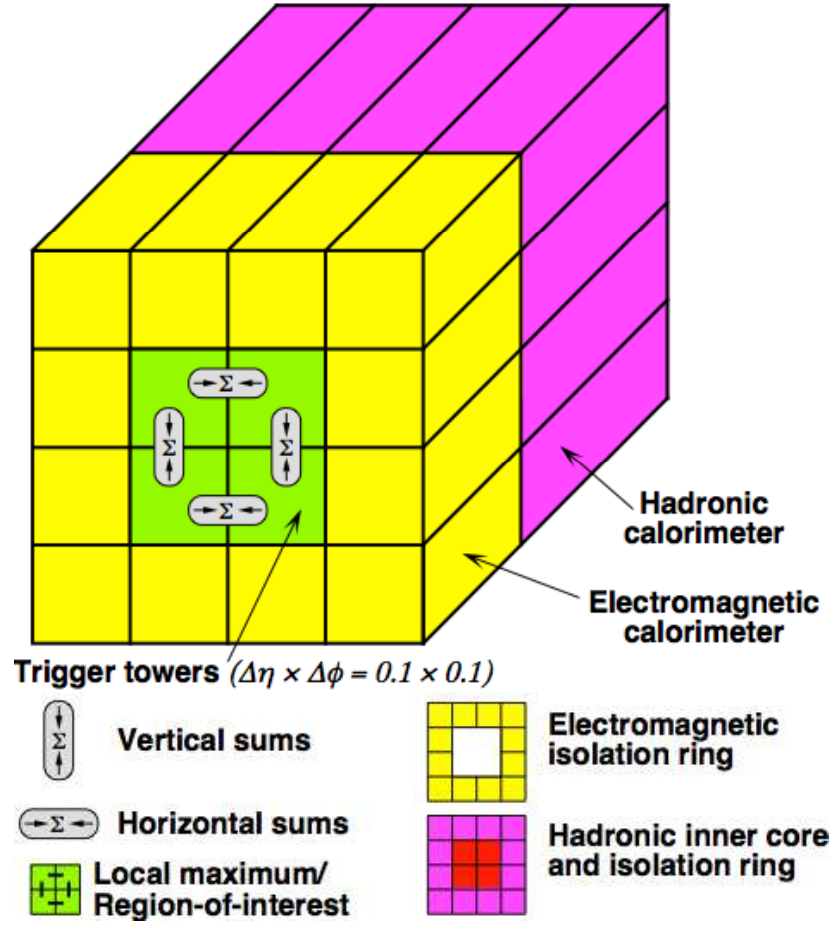
\includegraphics[width=\linewidth,height=\textheight,keepaspectratio]{trigger/trigger_towers}
            \caption{Structure of trigger towers and Regions of Interest \cite{L1_calo_run1}}
            \label{fig:trigger_towers}
        \end{figure}


        The Cluster Processor Module (CPM) exclusively uses the Barrel Calorimeters to function, and is primarily meant for rapid identification of electrons/photons and taus/hadrons.
        For either case, the CPM's first step is to check all possible $4 \times 4$ ``windows'' of trigger towers, identifying windows containing an isolated ``Region of Interest'' (RoI).
        Here, an RoI is defined as a $2 \times 2$ cluster of towers with an $E_T$ sum that is a relative maximum compared to surrounding towers.
        This $2 \times 2$ RoI is the center of the $4 \times 4$ window (see figure \ref{fig:trigger_towers}).
        Windows are considered as passing the CPM trigger if the RoI satisfies an isolation requirement, meaning that the 12 towers surrounding that core fall \textit{below} a predefined $E_T$ ``isolation threshold'' value.
        Electrons and photons are then separated from taus and hadrons by the fact that the latter group penetrates into the HCal barrel, while the former group stays highly contained to the ECal.

        Expanding out, the Jet/Energy Processing Module (JEM, or sometimes JEP) makes use of the calorimeter barrels and endcaps, as well as the FCAL, though it does not distinguish between the ECal and HCal.
        The JEM further reduces the granularity under consideration, with a basic unit of data collection being $2 \times 2$ collections of trigger towers called ``jet elements'', resulting in a minimum resolution of $0.2 \times 0.2$ in $\Delta \eta \times \Delta \phi$.
        Like the CPM, the JEM runs its trigger conditions on windows of multiple jet elements that must be based around a $2 \times 2$ RoI core (which is a local $E_T$ maximum).
        Unlike the CPM, these windows can vary in size.
        Primarily, the JEM is intended to perform hit multiplicity counting as well as assist the Extended Cluster Merger Modules (CMX) in carrying out the final jet multiplicity and $E_T$ sums \cite{L1_calo_run1}\cite{trigger_run2}.
        When these conditions, alongside those performed in the Muon trigger, are completed, the event is passed along to the HLT.


\FloatBarrier
    \subsection{High Level Trigger}

        After the L1 Trigger has reduced the event rate to 100 kHz, the software-based High Level Trigger is used to further reduce the event rate to the final output of \textasciitilde 1 kHz.
        Located in the SCX1 building (figure \ref{fig:facilities}) at the surface of P1 (again to minimize latency), the HLT uses data from all detector elements to completely reconstruct the event as it occurred in ATLAS, and performs its selections based on this reconstructed event.
        Different physics processes and particles, known as physics ``signatures'', are reconstructed in different ways, and have different triggers based around them. 
        The main signatures used in ATLAS are: minimum bias signatures, electron/photons (Egamma), muons, jets, taus, missing transverse energy (MET), b-jets (as in jets from bottom quarks), and B-physics (as in B-hadrons).
        The process of reconstruction and the trigger algorithms applied to these reconstructed signatures are based on offline software algorithms which have been repurposed for online use.
        These offline algorithms are quite technical in nature, and are discussed further in Chapter \ref{chapter:reconstruction}.
        Once events have successfully passed both L1 and the HLT, they are finally distributed off-site for analysis by different physics groups.

        \begin{figure}[h]
            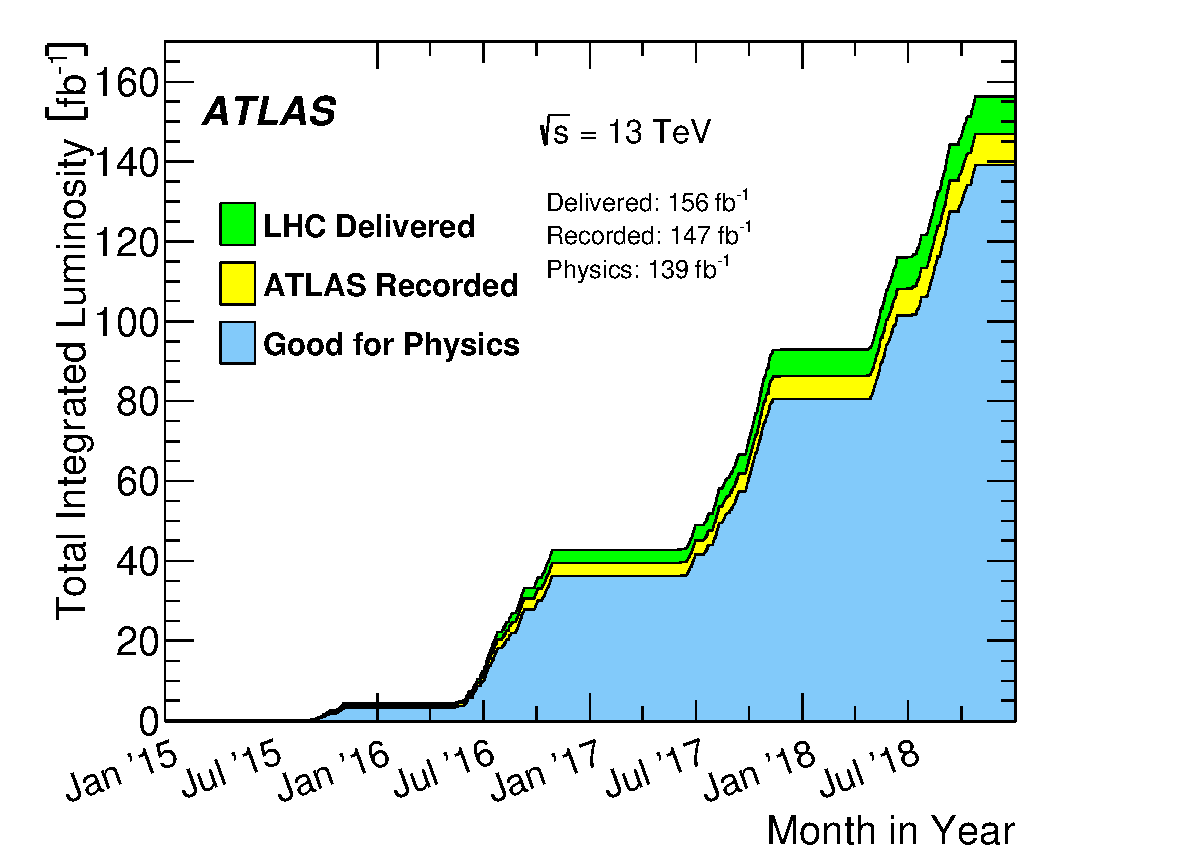
\includegraphics[width=\linewidth,height=\textheight,keepaspectratio]{trigger/data_delivered}
            \caption{Amount of data collected, in terms of integrated luminosity,
                through the Run2 data taking period\cite{data_quality}
                [TODO Steve this plot doesn't make any sense.
                This seems to imply that the trigger hardly throws away any events.
                Is that right?]}
            \label{fig:data_delivered}
        \end{figure}

        Over its three operational years, Run 2 has collected a total of 139 \ifb of data which has passed the online triggers
            (see figure \ref{fig:data_delivered}).
        Due to an inefficiency in the vertex reconstruction present during 2016,
            only 125.9 \ifb of that data are actually used in this analysis.
        Of that data, only a tiny portion is expected to be the actual di-Higgs signal event,
            which means further selection criteria will need to be applied.
        Understanding how the signal contribution is determined, and how these selections are optimized,
            requires understanding the second kind of data used for this analysis, Monte Carlo simulation data.


\FloatBarrier
\section{Monte-Carlo Simulation} \label{sec:mcsim}
    
    Currently, Monte-Carlo simulation is the most effective method of making predictions
        for how theoretical parameters should affect experimental observations in particle physics.
    The process for this analysis is a complex one, 
        consisting of three distinct software frameworks used to achieve a fully simulated output prediction.
    Their ultimate goal is to produce a faithful reproduction of how a collection of VBF \to HH processes would appear,
        were they to occur in data collected from ATLAS.
    The chain begins with pure theoretical simulation from MadGraph,
        the output of which is fed to a program called Pythia8,
        which in turn has its output run through the Geant4 simulation framework.
    Output from Geant4 is made to take the same form as if it came from the ATLAS hardware,
        at which point it can be processed in the same manner as real data and studied to make analysis decisions.


    \subsection{MadGraph}

    Madgraph is technically a meta-code, a program that creates a program,
        with the created program designed to simulate physics in the manner described by Madgraph.
    To do this, Madgraph needs a theory model, which consists of a lagrangian of the desired physics
        alongside input parameters such as coupling values and particle masses.
    The feynman rules are derived from the given lagrangian,
        which are in turn used to create the process's matrix elements (see Section \ref{sec:feyn_rules}).
    Feynman rules alone are sufficient to then produce tree-level calculations automatically.
    For NLO calculations, additional counterterms must be supplied by hand
        so that matrix element computations appropriately converge during loop integrations. 
    With these features supplied, MadGraph generates code specific to the supplied model,
        which in turn calculates and computes the matrix elements of the requested process\cite{madgraph}.
    A large number of events are produced using Monte Carlo techniques,
        each involving a different configuration of four momenta for the associated particles.
    These events represent a different point in the phase-space of the process,
        and a weight is assigned to each corresponding to its probability as calculated from the matrix element computation.
    The final collection of events is then output for use by later stages of the simulation process.

    %[cite TODO good christ the madgraph docs are garbage and now I have to cite a WEB FORUM post by some student who was ALSO commenting on how aweful the documentation for this stuff is... https://answers.launchpad.net/mg5amcnlo/+question/291534]

    \subsection{Pythia8}

    The final particles produced by MadGraph are often short-lived and unstable,
        and so require further simulation of their breakdown and decay.
    Pythia8 is the software responsible for this phase of the simulation. 
    By default, Pythia8 is entirely self-contained, and can generate physics processes entirely on its own.
    However, the processes available to it are limited,
        hence the need to first generate the bare interaction with MadGraph.
    Pythia8 operates in three stages: process generation, partonic activity handling, and hadronization.
    Process generation is the step which is taken over by MadGraph.
    The partonic stage addresses what happens to the parts of the proton \textit{not} involved in the immediate interaction (beam remnants),
        initial and final-state radiation of the final state particles, and inter-parton interactions.
    Following this is the hadronization stage, wherein final-state (but unstable)
        hadronic particles are extended through a cycle of decay, annihilation, and creation
        until a shower of stable hadronic matter remains.
    These steps are not fixed in Pythia's framework,
        and individual particles can transfer back and forth between these three stages
        as necessary to reach the stable state of the event as would be observed through a detector
        \cite{pythia}.
    The observation through a detector aspect then consitutes the final step of event simulation,
        which is handled by Geant4.

    \subsection{Geant4}

    Geant4 is a robust particle simulation framework,
        which seeks to provide a comprehensive simulation of how particles behave as they propagate through physical materials.
    The entire geometry of the material in question is specified in the Geant4 framework in terms of
        its specific shape, location, and material properties.
    For this analysis, that means a replica of the entire ATLAS detector,
        down to the copper wiring and individual metal bolts,
        has been meticulously crafted across a set of specification files Geant4 can read in.
    After specifying the geometry to simulate, individual events can be propagated through the materials.

    An event procedure starts with a set of final-state particles,
        either generated through one of Geant4's built-in processes,
        or provided to it from an external program (in this case, Pythia8).
    These particles are moved forward in small time steps, according to their associated four-momentum.
    As they encounter different materials,
        these time steps are adjusted to be longer or shorter depending on
        the expected mean-free path and radiation length of the particle.
    For every step in a particle's movement,
        Geant4 examines a wide variety of physics processes the particle can undergo,
        ranging across material scattering, radiation, decay, and so on.
    Particles are split, absorbed, and created as necessary,
        until all particles have either been absorbed by material
        or exited the physical scope of the simulation (e.g.\ muons escaping from ATLAS) \cite{geant4}.

    Geant4 additionally simulates the response of materials to these particle interactions,
        allowing energy and charge readouts to be simulated as they would be found within detector elements.
    The last step is to digitize these material responses to emulate the pixels and channels of a real detector.
    All of the event response information, as well as an abundance of \textit{truth} information related to the simulated particles,
        is exported to a data format identical in nature to that produced by the ATLAS trigger system.
    This simulated data can then be processed in the same manner as real data,
        allowing critical studies to be performed that in turn produce
        a far better understanding of the physics underlying the data.



    %MadGraph is used for producing simulated particle interactions based on the Feynman diagrams of the process.
    %Using a configuration of particle properties and interaction vertices,
    %    MadGraph is able to construct a tree-level formula akin to Equation \ref{eq:tree_level_invamp}.
    %It does this by using the provided configuration to prepare a list of Feynman rules,
    %    compose all tree-level diagrams that could result from those rules,
    %    and then perform the appropriate matrix element squared expansion.
    %Given a desired initial and final particle state,
    %    MadGraph can produce PDFs for the four-momentum of the final-state particles.
    %A collection of \textit{truth-level} simulated events can then be generated from MadGraph
    %    by sampling from these kinematic PDFs.

    %Although MadGraph does a fine job of generating output particles with kinematics resulting from a production process,
    %    in practice such particles rarely remain in such a state for very long.
    %Most particles, given any appreciable amount of time to propagate, will undergo some form of decay or radioactive emission.
    %Such processes occur randomly, and will often occur repeatedly
    %    (e.g.\ the products of a decay process can themselves undergo further decay).
    %Pythia8 is used to simulate these decay chains.
    %It uses a variety of built-in physics processes to inform the behavior of high-energy collision particle products.
    %This simulation is done entirely in a vacuum though, and one last program is required for full simulation.

    %Geant4 is responsible for the final step of event simulation,
    %    which is to simulate the propagation of particles through the physical hardware of ATLAS,
    %    and then simulate the detector response to this propagation.
    %A full three-dimensional simulation of ATLAS has been constructed within the Geant4 framework,
    %    modeling the exact dimensions and material composition of every component,
    %    be it an active detector material or an inactive support structure.
    %The particles and showers output by Pythia8 are propagated through the materials of the ATLAS machine by Geant4,
    %    with further modeling of showering and scattering effects.

